In the following chapter, I will introduce the \ac{PowerTAC} simulation. It's simulating a "liberalized" retail electrical energy market where multiple autonomous agents compete in different markets. Firstly, a retail market where agents, or \emph{brokers}, compete for numerous end-users through the offering of tariff contracts. Secondly, a wholesale market in which brokers buy and sell large amounts of electric energy to match their customers demands. This market allows brokers to place bids up to 24 hours in advance and each hour the broker has the ability to place new bids to correct for changes in their forecast models. Lastly, the balancing market which places relatively high costs on any broker that causes an imbalance in the system, giving incentives to the brokers to balance their own portfolios prior to the balancing operations. Figure ~\ref{fig:powertacoverview} summarizes this ecosystem.
\begin{figure}[!h]
    \centering
    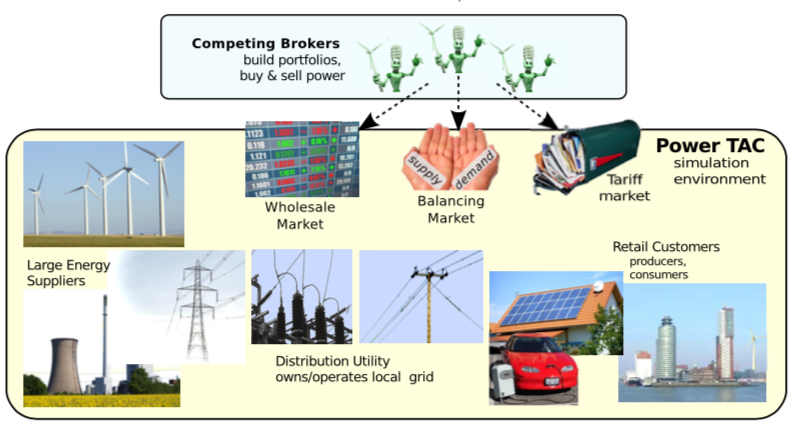
\includegraphics[width=0.6\textwidth]{powerTACScenarioOverview.png}
	%TODO check figure
	\caption{\ac{PowerTAC} overview of markets}
    \label{fig:powertacoverview}
\end{figure}

\section{Market concepts}

%OVERVIEW,Economical
The broker to be developed has to contest in a number of markets and handle a variety of customer types. While the \ac{PowerTAC} competition generates a fairly complex landscape, it mostly aims at economic complexity rather than modeling the technical underpinnings of the system. It therefore doesn't simulate any hardware but rather focuses on the different agents involved in the market.

%TIMESLOTS
The simulation emulates a time span of approximately 60 days with 1h time slot precision and accelerates this to 5 real-world seconds corresponding to each game-hour. The simulation emulates a time span of approximately 60 days with 1h time slot precision and accelerates this to 5 real-world seconds corresponding to each game-hour.


\subsection{Customer Market}

The foundation for any broker making profit is a sufficient amount of customers being subscribed to its tariffs. For this to occur, the broker must publish tariffs that are competitive as to attract customers. On the other hand, if the broker offers tariffs that lead to net losses, long term profit will not be possible. While the 2017 competition technically allowed for brokers to remain in the game despite offering highly underpriced tariffs that corrupted the simulation results, a proper broker must not pursue such strategies simply because of economical reasoning. %TODO verify 2017 corruption  

% - time energy, money, communication --> agent gets ability to choose freely across all dimensions? 
\subsection{Wholesale Market}
\subsection{Balancing Market}

\section{Broker concepts}
\subsection{Decision areas}
\subsection{Decision models}
\subsection{Past performances}

\section{Technology concepts}
\subsection{Server technologies}


